\documentclass{standalone}
\usepackage{tikz}
\usetikzlibrary{patterns, positioning}


\begin{document}
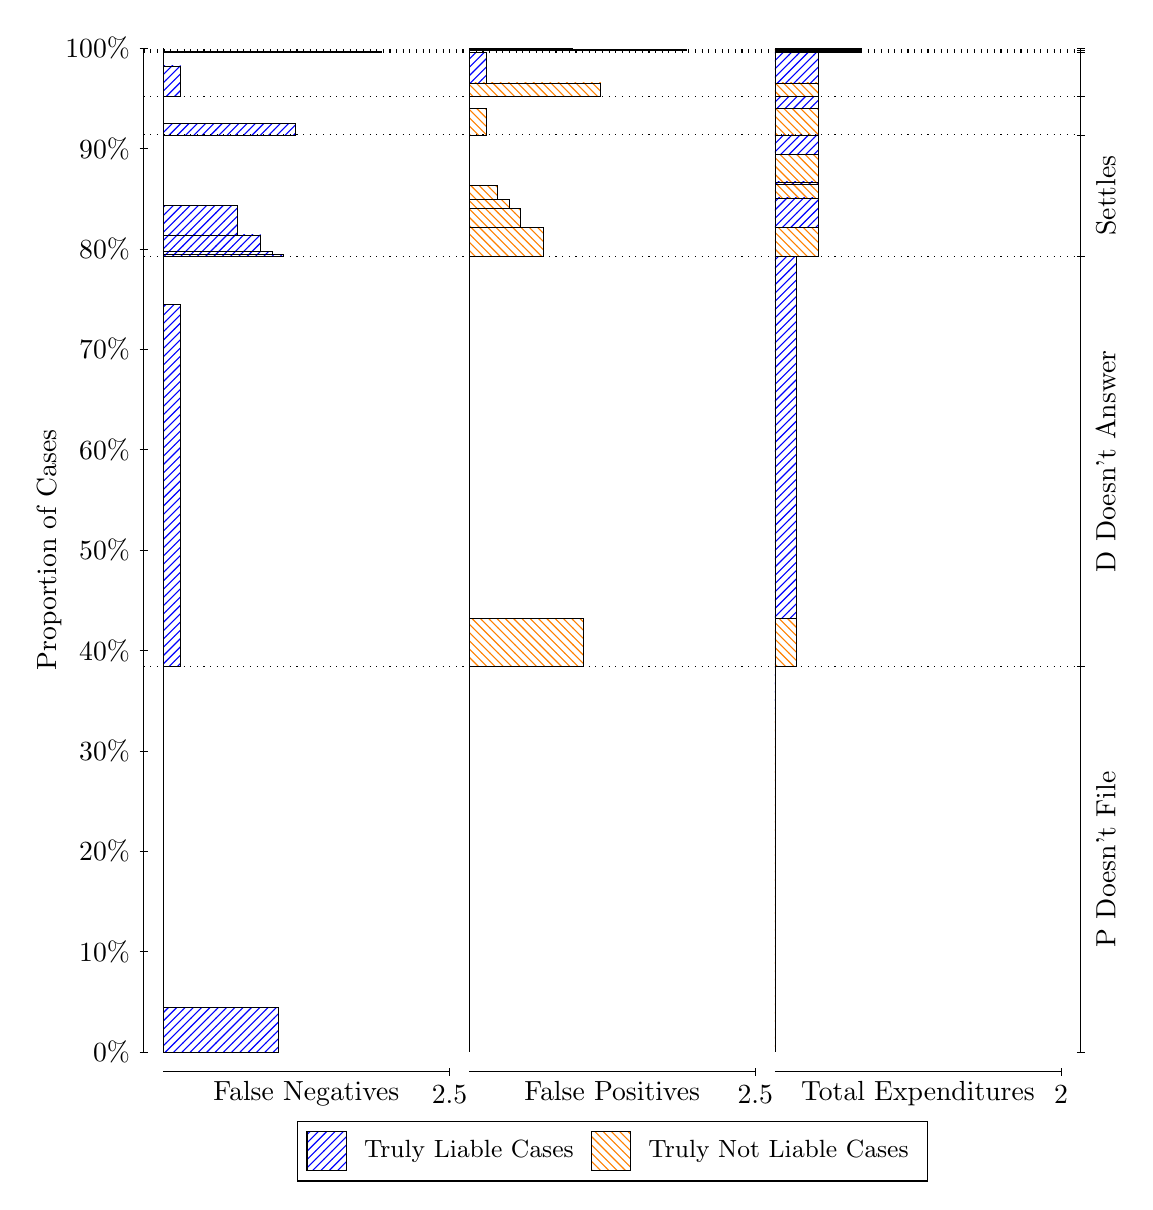
\begin{tikzpicture}
\draw[black, very thin] (1.5,1.75) -- (1.5,14.5);
\node[rotate=90, text=black, anchor=center] at (0.3, 8.125) {Proportion of Cases};
\draw[black, very thin] (1.45,1.75) -- (1.55,1.75);
\node[text=black, anchor=east] at (1.45, 1.75) {0\%};
\draw[black, very thin] (1.45,3.025) -- (1.55,3.025);
\node[text=black, anchor=east] at (1.45, 3.025) {10\%};
\draw[black, very thin] (1.45,4.3) -- (1.55,4.3);
\node[text=black, anchor=east] at (1.45, 4.3) {20\%};
\draw[black, very thin] (1.45,5.575) -- (1.55,5.575);
\node[text=black, anchor=east] at (1.45, 5.575) {30\%};
\draw[black, very thin] (1.45,6.85) -- (1.55,6.85);
\node[text=black, anchor=east] at (1.45, 6.85) {40\%};
\draw[black, very thin] (1.45,8.125) -- (1.55,8.125);
\node[text=black, anchor=east] at (1.45, 8.125) {50\%};
\draw[black, very thin] (1.45,9.4) -- (1.55,9.4);
\node[text=black, anchor=east] at (1.45, 9.4) {60\%};
\draw[black, very thin] (1.45,10.675) -- (1.55,10.675);
\node[text=black, anchor=east] at (1.45, 10.675) {70\%};
\draw[black, very thin] (1.45,11.95) -- (1.55,11.95);
\node[text=black, anchor=east] at (1.45, 11.95) {80\%};
\draw[black, very thin] (1.45,13.225) -- (1.55,13.225);
\node[text=black, anchor=east] at (1.45, 13.225) {90\%};
\draw[black, very thin] (1.45,14.5) -- (1.55,14.5);
\node[text=black, anchor=east] at (1.45, 14.5) {100\%};

\draw[black, very thin] (13.4,1.75) -- (13.4,14.5);
\draw[black, very thin] (13.35,1.75) -- (13.45,1.75);
\node[anchor=west] at (13.35, 1.75) {};
\draw[black, very thin] (13.35,6.6456) -- (13.45,6.6456);
\node[anchor=west] at (13.35, 6.6456) {};
\draw[black, very thin] (13.35,11.855) -- (13.45,11.855);
\node[anchor=west] at (13.35, 11.855) {};
\draw[black, very thin] (13.35,13.398) -- (13.45,13.398);
\node[anchor=west] at (13.35, 13.398) {};
\draw[black, very thin] (13.35,13.883) -- (13.45,13.883);
\node[anchor=west] at (13.35, 13.883) {};
\draw[black, very thin] (13.35,14.449) -- (13.45,14.449);
\node[anchor=west] at (13.35, 14.449) {};
\draw[black, very thin] (13.35,14.475) -- (13.45,14.475);
\node[anchor=west] at (13.35, 14.475) {};
\draw[black, very thin] (13.35,14.5) -- (13.45,14.5);
\node[anchor=west] at (13.35, 14.5) {};

\draw[black, very thin, pattern color=blue, pattern=north east lines] (1.75,1.75) rectangle (3.2033,2.3148);
\draw[black, very thin, pattern color=orange, pattern=north west lines] (1.75,2.3148) rectangle (1.75,6.6456);
\draw[black, very thin, pattern color=blue, pattern=north east lines] (1.75,6.6456) rectangle (1.968,11.248);
\draw[black, very thin, pattern color=orange, pattern=north west lines] (1.75,11.248) rectangle (1.75,11.855);
\draw[black, very thin, pattern color=blue, pattern=north east lines] (1.75,11.855) rectangle (3.276,11.882);
\draw[black, very thin, pattern color=blue, pattern=north east lines] (1.75,11.882) rectangle (3.1307,11.919);
\draw[black, very thin, pattern color=blue, pattern=north east lines] (1.75,11.919) rectangle (2.9853,12.128);
\draw[black, very thin, pattern color=blue, pattern=north east lines] (1.75,12.128) rectangle (2.6947,12.5);
\draw[black, very thin, pattern color=orange, pattern=north west lines] (1.75,12.5) rectangle (1.75,13.398);
\draw[black, very thin, pattern color=blue, pattern=north east lines] (1.75,13.398) rectangle (3.4213,13.545);
\draw[black, very thin, pattern color=orange, pattern=north west lines] (1.75,13.545) rectangle (1.75,13.883);
\draw[black, very thin, pattern color=blue, pattern=north east lines] (1.75,13.883) rectangle (1.968,14.274);
\draw[black, very thin, pattern color=orange, pattern=north west lines] (1.75,14.274) rectangle (1.75,14.449);
\draw[black, very thin, pattern color=blue, pattern=north east lines] (1.75,14.449) rectangle (4.5113,14.461);
\draw[black, very thin, pattern color=orange, pattern=north west lines] (1.75,14.461) rectangle (1.75,14.475);
\draw[black, very thin, pattern color=orange, pattern=north west lines] (1.75,14.475) rectangle (1.75,14.487);
\draw[black, very thin, pattern color=blue, pattern=north east lines] (1.75,14.487) rectangle (1.75,14.5);
\draw[black, very thin, pattern color=orange, pattern=north west lines] (5.6333,1.75) rectangle (5.6333,6.0809);
\draw[black, very thin, pattern color=blue, pattern=north east lines] (5.6333,6.0809) rectangle (5.6333,6.6456);
\draw[black, very thin, pattern color=orange, pattern=north west lines] (5.6333,6.6456) rectangle (7.0867,7.253);
\draw[black, very thin, pattern color=blue, pattern=north east lines] (5.6333,7.253) rectangle (5.6333,11.855);
\draw[black, very thin, pattern color=orange, pattern=north west lines] (5.6333,11.855) rectangle (6.578,12.227);
\draw[black, very thin, pattern color=orange, pattern=north west lines] (5.6333,12.227) rectangle (6.2873,12.461);
\draw[black, very thin, pattern color=orange, pattern=north west lines] (5.6333,12.461) rectangle (6.142,12.577);
\draw[black, very thin, pattern color=orange, pattern=north west lines] (5.6333,12.577) rectangle (5.9967,12.754);
\draw[black, very thin, pattern color=blue, pattern=north east lines] (5.6333,12.754) rectangle (5.6333,13.398);
\draw[black, very thin, pattern color=orange, pattern=north west lines] (5.6333,13.398) rectangle (5.8513,13.736);
\draw[black, very thin, pattern color=blue, pattern=north east lines] (5.6333,13.736) rectangle (5.6333,13.883);
\draw[black, very thin, pattern color=orange, pattern=north west lines] (5.6333,13.883) rectangle (7.3047,14.058);
\draw[black, very thin, pattern color=blue, pattern=north east lines] (5.6333,14.058) rectangle (5.8513,14.449);
\draw[black, very thin, pattern color=orange, pattern=north west lines] (5.6333,14.449) rectangle (5.6333,14.463);
\draw[black, very thin, pattern color=blue, pattern=north east lines] (5.6333,14.463) rectangle (5.6333,14.475);
\draw[black, very thin, pattern color=orange, pattern=north west lines] (5.6333,14.475) rectangle (8.3947,14.487);
\draw[black, very thin, pattern color=blue, pattern=north east lines] (5.6333,14.487) rectangle (6.9413,14.5);
\draw[black, very thin, pattern color=orange, pattern=north west lines] (9.5167,1.75) rectangle (9.5167,6.0809);
\draw[black, very thin, pattern color=blue, pattern=north east lines] (9.5167,6.0809) rectangle (9.5167,6.6456);
\draw[black, very thin, pattern color=orange, pattern=north west lines] (9.5167,6.6456) rectangle (9.7892,7.253);
\draw[black, very thin, pattern color=blue, pattern=north east lines] (9.5167,7.253) rectangle (9.7892,11.855);
\draw[black, very thin, pattern color=orange, pattern=north west lines] (9.5167,11.855) rectangle (10.062,12.227);
\draw[black, very thin, pattern color=blue, pattern=north east lines] (9.5167,12.227) rectangle (10.062,12.598);
\draw[black, very thin, pattern color=orange, pattern=north west lines] (9.5167,12.598) rectangle (10.062,12.775);
\draw[black, very thin, pattern color=blue, pattern=north east lines] (9.5167,12.775) rectangle (10.062,12.801);
\draw[black, very thin, pattern color=orange, pattern=north west lines] (9.5167,12.801) rectangle (10.062,13.152);
\draw[black, very thin, pattern color=blue, pattern=north east lines] (9.5167,13.152) rectangle (10.062,13.398);
\draw[black, very thin, pattern color=orange, pattern=north west lines] (9.5167,13.398) rectangle (10.062,13.736);
\draw[black, very thin, pattern color=blue, pattern=north east lines] (9.5167,13.736) rectangle (10.062,13.883);
\draw[black, very thin, pattern color=orange, pattern=north west lines] (9.5167,13.883) rectangle (10.062,14.058);
\draw[black, very thin, pattern color=blue, pattern=north east lines] (9.5167,14.058) rectangle (10.062,14.449);
\draw[black, very thin, pattern color=orange, pattern=north west lines] (9.5167,14.449) rectangle (10.607,14.463);
\draw[black, very thin, pattern color=blue, pattern=north east lines] (9.5167,14.463) rectangle (10.607,14.475);
\draw[black, very thin, pattern color=orange, pattern=north west lines] (9.5167,14.475) rectangle (10.607,14.487);
\draw[black, very thin, pattern color=blue, pattern=north east lines] (9.5167,14.487) rectangle (10.607,14.5);
\draw[black, dotted] (1.5,6.6456) -- (13.4,6.6456);
\draw[black, dotted] (1.5,11.855) -- (13.4,11.855);
\draw[black, dotted] (1.5,13.398) -- (13.4,13.398);
\draw[black, dotted] (1.5,13.883) -- (13.4,13.883);
\draw[black, dotted] (1.5,14.449) -- (13.4,14.449);
\draw[black, dotted] (1.5,14.475) -- (13.4,14.475);
\draw[black, very thin] (1.75,1.5) -- (5.3833,1.5);
\node[text=black, anchor=north] at (3.5667, 1.5) {False Negatives};
\draw[black, very thin] (5.3833,1.45) -- (5.3833,1.55);
\node[text=black, anchor=north] at (5.3833, 1.45) {2.5};

\draw[black, very thin] (5.6333,1.5) -- (9.2667,1.5);
\node[text=black, anchor=north] at (7.45, 1.5) {False Positives};
\draw[black, very thin] (9.2667,1.45) -- (9.2667,1.55);
\node[text=black, anchor=north] at (9.2667, 1.45) {2.5};

\draw[black, very thin] (9.5167,1.5) -- (13.15,1.5);
\node[text=black, anchor=north] at (11.333, 1.5) {Total Expenditures};
\draw[black, very thin] (13.15,1.45) -- (13.15,1.55);
\node[text=black, anchor=north] at (13.15, 1.45) {2};

\node[text=black, centered, rotate=90] at (13.72, 4.1978) {P Doesn't File};
\node[text=black, centered, rotate=90] at (13.72, 9.2503) {D Doesn't Answer};
\node[text=black, centered, rotate=90] at (13.72, 12.627) {Settles};





\draw (7.449999999999999,1.5) node[draw=none] (baseCoordinate) {};
\begin{scope}[align=center]
        \matrix[scale=0.5, draw=black, below=0.5cm of baseCoordinate, nodes={draw}, column sep=0.1cm]{
            \node[rectangle, draw, minimum width=0.5cm, minimum height=0.5cm, pattern color=blue, pattern=north east lines] {}; &
            \node[draw=none, font=\small, text=black] (B) {Truly Liable Cases}; &
            \node[rectangle, draw, minimum width=0.5cm, minimum height=0.5cm, pattern color=orange, pattern=north west lines] {}; &
            \node[draw=none, font=\small, text=black] (B) {Truly Not Liable Cases}; \\
            };
\end{scope}

\end{tikzpicture}
\end{document}